%% This is file `elsarticle-template-1-num.tex',
%%
%% Copyright 2009 Elsevier Ltd
%%
%% This file is part of the 'Elsarticle Bundle'.
%% ---------------------------------------------
%%
%% It may be distributed under the conditions of the LaTeX Project Public
%% License, either version 1.2 of this license or (at your option) any
%% later version.  The latest version of this license is in
%%    http://www.latex-project.org/lppl.txt
%% and version 1.2 or later is part of all distributions of LaTeX
%% version 1999/12/01 or later.
%%
%% Template article for Elsevier's document class `elsarticle'
%% with numbered style bibliographic references
%%
%% $Id: elsarticle-template-1-num.tex 149 2009-10-08 05:01:15Z rishi $
%% $URL: http://lenova.river-valley.com/svn/elsbst/trunk/elsarticle-template-1-num.tex $
%%
\documentclass[final, 12pt]{elsarticle}

%% Use the option review to obtain double line spacing
%% \documentclass[preprint,review,12pt]{elsarticle}

%% Use the options 1p,twocolumn; 3p; 3p,twocolumn; 5p; or 5p,twocolumn
%% for a journal layout:
%% \documentclass[final,1p,times]{elsarticle}
%% \documentclass[final,1p,times,twocolumn]{elsarticle}
%% \documentclass[final,3p,times]{elsarticle}
%% \documentclass[final,3p,times,twocolumn]{elsarticle}
%% \documentclass[final,5p,times]{elsarticle}
%% \documentclass[final,5p,times,twocolumn]{elsarticle}

%% The graphicx package provides the includegraphics command.
\usepackage{graphicx}
%% The amssymb package provides various useful mathematical symbols
\usepackage{amssymb}
%% The amsthm package provides extended theorem environments
%% \usepackage{amsthm}

%% The lineno packages adds line numbers. Start line numbering with
%% \begin{linenumbers}, end it with \end{linenumbers}. Or switch it on
%% for the whole article with \linenumbers after \end{frontmatter}.
\usepackage{lineno}

%% natbib.sty is loaded by default. However, natbib options can be
%% provided with \biboptions{...} command. Following options are
%% valid:

%%   round  -  round parentheses are used (default)
%%   square -  square brackets are used   [option]
%%   curly  -  curly braces are used      {option}
%%   angle  -  angle brackets are used    <option>
%%   semicolon  -  multiple citations separated by semi-colon
%%   colon  - same as semicolon, an earlier confusion
%%   comma  -  separated by comma
%%   numbers-  selects numerical citations
%%   super  -  numerical citations as superscripts
%%   sort   -  sorts multiple citations according to order in ref. list
%%   sort&compress   -  like sort, but also compresses numerical citations
%%   compress - compresses without sorting
%%
%% \biboptions{comma,round}

% \biboptions{}

\journal{Indian Semantics and Ontology: HSS325}

\begin{document}

\begin{frontmatter}

%% Title, authors and addresses

\title{An Ontology for a Section of the \textit{Ashtadhyayi}: A Final Report}

%% use the tnoteref command within \title for footnotes;
%% use the tnotetext command for the associated footnote;
%% use the fnref command within \author or \address for footnotes;
%% use the fntext command for the associated footnote;
%% use the corref command within \author for corresponding author footnotes;
%% use the cortext command for the associated footnote;
%% use the ead command for the email address,
%% and the form \ead[url] for the home page:
%%
%% \title{Title\tnoteref{label1}}
%% \tnotetext[label1]{}
%% \author{Name\corref{cor1}\fnref{label2}}
%% \ead{email address}
%% \ead[url]{home page}
%% \fntext[label2]{}
%% \cortext[cor1]{}
%% \address{Address\fnref{label3}}
%% \fntext[label3]{}


%% use optional labels to link authors explicitly to addresses:
%% \author[label1,label2]{<author name>}
%% \address[label1]{<address>}
%% \address[label2]{<address>}

\author{Alok Debnath}

\address{20161122 \\
  {\tt alok.debnath@research.iiit.ac.in}}

\begin{abstract}
 In this report, I demonstrate the development of an ontology for a subset of the words present in Panini's \emph{Ashtadhyayi}. The set of words provided were in fact not related to one another, rather were in lexicographic ordering. This handicap made the creation of this ontology an interesting exercise. I did not use existing knowledge graphs, rather used a simple approach of an abstract notion of semantic role of the words. This allows for a simple and flexible ontology, but it also has the drawbacks of not representing polysemy and some corner cases based on the definitions of each category.
\end{abstract}

\begin{keyword}
Sanskrit \sep Ontology \sep Ashtadhyayi
%% keywords here, in the form: keyword \sep keyword

%% MSC codes here, in the form: \MSC code \sep code
%% or \MSC[2008] code \sep code (2000 is the default)

\end{keyword}

\end{frontmatter}

%% main text
\section{Introduction}
\label{intro}

Natural language ontology is a branch of both metaphysics and linguistic semantics. Its aim is to uncover the ontological categories, notions, and structures that are implicit in the use of natural language, that is, the ontology that a speaker accepts when using a language \cite{moltmann2017natural}. Sanskrit has a very rich tradition of arrangement and representation of meanings, as has been demonstrated in the \emph{Nyaya} and \emph{Vaisheshika} schools.

More recently, the work done in knowledge representation in natural language processing has led to the conception and development of knowledge graphs and networks \citep{huang2010ontology}. While a consequence of semantic representation of knowledge, these are not strictly ontological in nature \citep{bateman1997theoretical}, as they do not show the hierarchical classification of the meanings of words based on their use and intrinsic properties. Rather, these representations are arrangements of words and the relations between those words as one might find them in a lexicon. Some examples of these types of representations include WordNet \citep{miller1995wordnet}, VerbNet \citep{schuler2005verbnet} and ConceptNet \citep{liu2004conceptnet}.

In this project, our aim was to select a set of about a hundred Paṇinian semantic conditions used in either the Dhatupaṭha or in the Aṣṭhadhyayi and construct a formal semantic network, investigate various existing formal semantic networks and select one to use as the model or framework for your network of Paṇinian semantic conditions. The semantic conditions chosen were from the Astahayi. I investigated the Vaisheshika ontology (categories of \emph{padartha}; section \ref{sec: vai_ontology}) and the network WordNet (section \ref{sec: wordnet}). However, given that the words in the subset I chose were lexicographically chosen, it would be futile to use a description as large as the Vaisheshika ontology. On the other hand, the words were not related enough to use a lexical arrangement such as WordNet, nor were they conceptually intertwined as the ConceptNet, which is why I chose to restructure a subset of the Vaisheshika ontology to suit the words I chose. This process has been described in Section \ref{sec: my_onto}

\section{Vaisheshika ontology}
\label{sec: vai_ontology}

\begin{figure}[t]
    \centering
    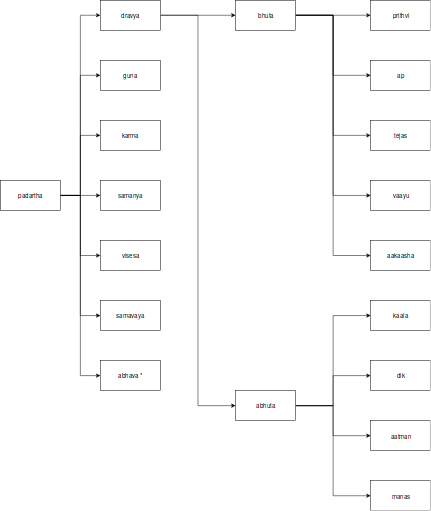
\includegraphics[width=350pt, height=350pt]{Ontology.png}
    \caption{The Vaisheshika ontology}
    \label{fig: vai_onto_pic}
\end{figure}

The most basic concept in the Vaisheshika ontology is that of \emph{padartha}. The word padartha is a sandhi of the words \emph{pada}, which means word and \emph{arhta} which translates to meaning. Originally, the word pada implies that form of a word which can be used in a sentence, including its inflectional changes. Padartha therefore means "the meaning or referent of words" \cite{daniel1951materials}.

Padartha is the basic unit of the ontology of both, the Nyaya and the Vaisheshika ontologies. The original Vaishseshka ontology categorizes the padarthas into six categories \citep{matilal1977nyaya}: 
\begin{itemize}
    \item \emph{dravya} (substance): This semantic category is defined as those concepts which are represented as objects or substances. In these substances, there are those which can be perceived by one or a combination of senses, as well as the objects of intellectual or logical existence, with no "real" or perceivable manifestation.
    
    \item \emph{guṇa} (quality): A guna is a quality or a property of substances. A guna is not capable of independent existence, as its function is only of describing the properties or qualities of substances, activities and other gunas. There are 17 types of gunas in the original \emph{Vaisheshika sutra}, while later authors have added 7 more. 
    
\item \emph{karma} (activity): A karma is defined as a transient feature of a substance. Like gunas, karmas do not have a separate existence, and are only manifested by their association to the substances. Karma are only associated with perceivable objects and substances
    
    \item \emph{samanya} (generality): Since there are plurality of substances, there will be relations among them. When a property is found common to many substances, it is called samanya.
    
    \item \emph{visheṣha} (particularity): While there is plurality, there is a difference between individual substances, that help identify them differently. When a property is found different between two similar objects, it is called vishesha.
    
    \item \emph{samavaya} (inherence): The relation between the cause and effect is not identified or percieved directly. However, there is a relation between the states of related objects, which is represented by samavaya. 
\end{itemize}

The later Vaisheshikas introduced the concept of \emph{abhaava} or absence, which was not represented as any of the above. This was done because each of the above categories can be referenced even in their absence, therefore making it necessary to include it in the ontology. A diagrammatic representation of the Vaisheshika ontology is given in figure \ref{fig: vai_onto_pic}. For brevity, the types of guna are not represented in the figure.

\section{WordNet}
\label{sec: wordnet}

WordNet is an online lexical database, which shows the relations between the entries. These relations are based on the part of speech of the words. One of the most important contributions of WordNet is that it disambiguates the senses of each of the polysemous words in the network. This makes establishing semantic relations between words easier, as each word (with its sense ID) means exactly one thing.

\begin{figure}
    \centering
    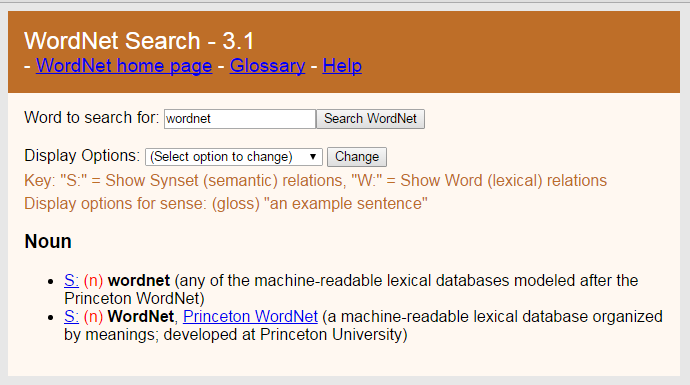
\includegraphics[width=13.5cm]{WordNet.png}
    \caption{WordNet UI}
    \label{fig: wordnet-ui}
\end{figure}

Originally, WordNet has relations which are defined below \citep{miller1995wordnet}:
\begin{itemize}
    \item Synonymy: Synonymy is the relation that establishes that two words mean either exactly or roughly the same. This is based on their meaning in the dictionary. Note that "word" refers only to one particular sense of that word. Synonymy is considered a basic relation, primarily because WordNet bases the concept of synsets as the basic relation of the word senses. A synset of a word is a set of all the words which are synonyms of it. This is primary is sense disambiguation. Synonymy is appplied to all the parts of speech in WordNet, which are nouns, adjectives, verbs and adverbs. 
    \item Antonymy: Antonymy is the relation that establishes that two words are opposite. The opposite is based on the synset of the word, such that the synset of a word are antonyms of the synset of its antonym. Antonyms are also valid for all the parts of speech.
    \item Hyponymy: The subordinate relationship, a hyponym of a word denotes the 'type-of' relationship between two words (if A is a hyponym of B, then A is a type of B). This is a relationship restricted to nouns.  
    \item Hypernymy: The superordinate relationship is called the hypernymy relationship. The hypernymy relationship is the 'class-of' relationship between two words. Hypernymy is the opposite of the hyponymy relationship.
    \item Meronymy: Meronymy is a complex semantic relation. WordNet distinguishes component, substantive and member parts as the meronym relation. Therefore, a meronym can be considered as a 'part-of' relationship.
    \item Holonymy: Holonymy is the opposite of meronymy, which can be considered the 'whole-of' or 'class-of' relationship. Both meronymy and holonymy are relationships that apply to nouns only.
    \item Troponymy: Troponyms are verb-verb relationships, where the verbs are similar actions to each other, or can be used in a similar context. Troponymy are similar to homoymy, but can be based on the specificity of the use of the verb.
    \item Entailment: An entailment relationship is a verb-verb relationship that denotes a tatuological relationship between one action performed by one participant which directly implies that another action is being performed by another participant of the former action. These are quite common in transitive verb pairs
\end{itemize}

\begin{figure}
    \centering
    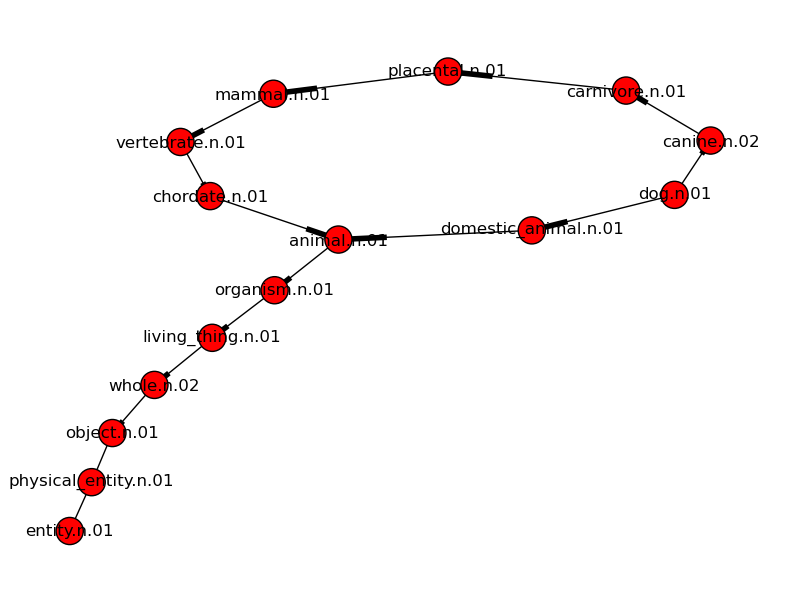
\includegraphics[width=13.5cm]{GraphWordNet.png}
    \caption{A Graphical Representation of a WordNet Snippet}
    \label{fig: wordnet-graph}
\end{figure}

Figure \ref{fig: wordnet-graph} is a graphical representation of some a snippet of the WordNet structure, the nodes representing the word senses, while the edges represent the relation of synonymy. Note that WordNet is a fully connected hypergraph, which means that it is possible to represent only one relation as a graph. This hypergraph structure has been used in multiple other projects, as WordNet has inspired multiple other knowledge representations including BableNet, a very large semantic network made by combining WordNet and the Wikipedia articles hypergraph \citep{navigli2010babelnet}, VerbNet, a comprehensive lexicon of verbs and their relations \citep{schuler2005verbnet}, Freebase \citep{bollacker2008freebase} and DBPedia \citep{auer2007dbpedia}.

\section{Ontology for this Project}
\label{sec: my_onto}

The ontology used for this project is an adaptation of the Vaisheshika ontology, which is based on the words chosen from the Ashtadhyayi. 

\subsection{Challenges in Ontology Choice}

The semantic conditions chosen for the project were lexicographically chosen from the Ashtadhyayi. Therefore, while I would have wanted to implement a word oriented lexical resource similar to WordNet and added more conceptual information on it, it was not possible to do so, simply because such a graph would be too sparse to represent any useful information. The Vaisheshika ontology, however, suited the words chosen.

It must be noted that the Vaisheshika ontology is very elaborate in its classification of words, as it does so for a large portion of the Sanskrit language. However, this was not the case with the I had to develop. The words chosen to represent the various classifications in the ontology were not chosen from the Ashtadhyayi conditions, they are English classes, as no such semantic constraints could be created otherwise. Therefore a very contracted and modified classification of words is presented in this project. 

\subsection{Ontology Design}

\begin{figure}
    \centering
    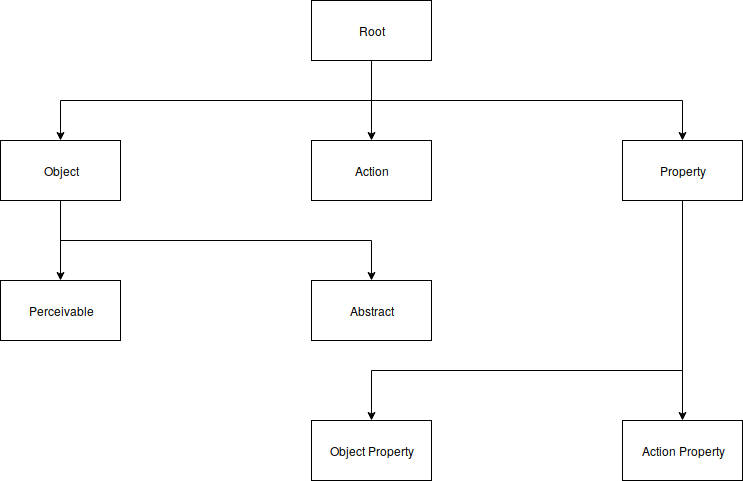
\includegraphics[width=13.5cm, height=10cm]{MyOntology.png}
    \caption{The Structure of my Ontology}
    \label{fig: my-ontology}
\end{figure}

I have designed a simple ontology, as shown in the figure \ref{fig: my-ontology}. The semantic categorization of words is based on the nature of their existence, and based on their meanings according to that. The meanings of the chosen words were originally chosen from the Monier-Williams Sanskrit to English Dictionary \citep{monier1964sanskrit}, verified from the Ashtadhyayi of Panini \citep{paṇini1962ashtadhyayi}. The most basic unit of the ontology is called an 'entity'. Each entity has a form (which can be dependent on the encoding and the type of font) and a meaning as stored in the above references. An example of this basic concept is provided below in figure \ref{fig: example}.

\begin{figure}
    \centering
    \begin{verbatim}
    <entity>
        <form> Silpin </form>
        <meaning> belonging to or skilled in art </meaning>
    </entity>
    \end{verbatim}
    \caption{Basic XML notation}
    \label{fig: example}
\end{figure}

The structure of the ontology is as follows (refer figure \ref{fig: my-ontology}):
\begin{itemize}
    \item Object: An object is similar to the category of substance in the original Vaisheshika ontology. A member of a class object has an independent existence, which is intransient. An object can be modified by a property, and there is a link between the property and the object of modifier-modified. This is subclassified in a manner similar to the Vaisheshika definition of \emph{artha} and \emph{budhyapeksham}, except very particularly for objects only.
    \begin{itemize}
        \item Perceivable: A perceivable object is one which can be cognized by one or a combination of the senses. While the nomenclature of a perceivable object (and its properties) are abstractly defined, it serves as a referent to an entity which can be 
        \item Abstract: An abstract object is an intellectually cognizable entity with no perceivable manifestation. Thoughts, ideas, sentience and such concepts are classified as abstract objects.
    \end{itemize}
    \item Action: An action is a transient property of an object, on the basis of which it undergoes some change in its properties. An object can be said to participate in or perform an action (irrespective of its sentience).
    \item Property: A property is an intransient modifier of an object or action. There are entities that describe the property of the object which are not inherent to the object itself. I also include in this category entities which describe the nature of an action.
\end{itemize}

This ontology, while not entirely complete, was enough to categorize all the words of the chosen section of the Ashtadhyayi.

\section{Conclusion}

The semantic conditions I have chosen are very broadly defined, and therefore served to classify most words into one category. There are exceptions, which are as follows:
\begin{itemize}
    \item A entity can denote an action while being an abstract object. Since the dictionary wasn't based on parts of speech, distinguishing this was difficult. It is the semantic conditions that explain which possible affixes can be applied to the word form, which was used to solve this.
    \item A property can describe or modify both an action and an object. Since actions and abstract objects can be modified by a property. This was still difficult to determine, and the Ashtadhyayi translations are too difficult to read and understand, compounding the problem.
\end{itemize}

The ontological structure however, is fairly extensible. The XML structure can be given attributes for further description. However, extending the ontology will make it similar to the Vaisheshika ontology.

\bibliographystyle{model1-num-names}
\bibliography{sample.bib}


\end{document}